\documentclass[a4paper]{report}
\usepackage{graphicx}

\title{ A Survey on IoT Based Smart City}
\author{Israt Jahan Joya (160239) \\ A. K. M. Fahim Rahman (160215)}

\begin{document}
	
	\maketitle
	
	
	
	\section*{1. Abstract}
	The Internet of Things (IoT) is a system of interrelated computing devices, mechanical and digital machines, objects, animals or people that are provided with unique identifiers and the ability to transfer data over a network without requiring human-to-human or human-to-computer interaction. Building a general architecture for the IoT is a very complex task because of the extremely use of large variety of devices, link layer technologies, and services that may be involved in that system. In this paper we have tried to make a survey on Smart Cities. We have mainly focused on Sound Pollution, waste management, electricity loss problem and the solution techniques.  
	\section*{2. Introduction}
	The Internet of Things (IoT) is a recent communication paradigm that envisions a near future, in which the objects of everyday life will be equipped with microcontrollers, transceivers for digital communication, and suitable protocol stacks that will make them able to communicate with one another and with the users, becoming an integral part of the Internet [1]. The IoT concept, hence, aims at making the Internet even more immersive and pervasive. Furthermore, by enabling easy access and interaction with a wide variety of devices such as, for instance, home appliances, surveillance cameras, monitoring sensors, actuators, displays, vehicles, and so on, the IoT will foster the development of a number of applications that make use of the potentially enormous amount and variety of data generated by such objects to provide new services to citizens, companies, and public administrations. This paradigm indeed finds application in many different domains, such as home automation, industrial automation, medical aids, mobile healthcare, elderly assistance, intelligent energy management and smart grids, automotive, traffic management, and many others [2].
	However, such a heterogeneous field of application makes the
	identification of solutions capable of satisfying the requirements
	of all possible application scenarios a formidable challenge. This
	difficulty has led to the proliferation of different and, sometimes, incompatible proposals for the practical realization of IoT systems. Therefore, from a system perspective, the realization of an IoT network, together with the required backend network services and devices, still lacks an established best practice because of its novelty and complexity. In addition to the technical
	difficulties, the adoption of the IoT paradigm is also hindered
	by the lack of a clear and widely accepted business model that
	can attract investments to promote the deployment of these
	technologies [3].
	The objective of this paper is to discuss about smart city and the solution technique of some problems like sound pollution problem, electricity loss problem, and waste management system of a smart city. We have tried to find the answers of following questions \\
	- By which technique sound pollution problem, electricity loss problem can be solved?\\
	- Which technique can maintain waste management system smartly?
	
	The rest of the paper is organized as follows. In section 2 we have discussed about smart city and its features. Then in section 3 we have discussed the solution techniques of sound pollution problem, electricity loss problem and also discussed about waste management system. Section 4 discussed about future research possibilities for making smart cities cost efficiently, section 5 discussed answers to the research question and finally section 6 concludes the paper with final remarks. 
	\section*{3. Smart City Concept and Services:}
	According to Pike Research on Smart Cities, [10] the Smart City
	market is estimated at hundreds of billion dollars by 2020, with
	an annual spending reaching nearly 16 billion. This market
	springs from the synergic interconnection of key industry and service sectors, such as Smart Governance, Smart Mobility,
	Smart Utilities, Smart Buildings, and Smart Environment. These
	sectors have also been considered in the European Smart Cities
	project (http://www.smart-cities.eu) to define a ranking criterion
	that can be used to assess the level of “smartness” of European
	cities. Nonetheless, the Smart City market has not really taken off yet, for a number of political, technical, and financial barriers [4]. Under the political dimension, the primary obstacle is the
	attribution of decision-making power to the different stakeholders. A possible way to remove this roadblock is to institutionalize the entire decision and execution process, concentrating the strategic planning and management of the smart city aspects into a single, dedicated department in the city [5]. Lets take a look few important paradigm of IoT Based Smart City.\\
	Waste Management: Waste management is a primary issue in
	many modern cities, due to both the cost of the service and the
	problem of the storage of garbage in landfills. A deeper penetration of ICT solutions in this domain, however, may result in
	significant savings and economical and ecological advantages.
	For instance, the use of intelligent waste containers, which detect
	the level of load and allow for an optimization of the collector
	trucks route, can reduce the cost of waste collection and improve
	the quality of recycling [6].3 To realize such a smart waste
	management service, the IoT shall connect the end devices, i.e.,
	intelligent waste containers, to a control center where an optimization software processes the data and determines the optimal management of the collector truck fleet. \\
	Smart Lighting: In order to support the 20-20-20 directive, the
	optimization of the street lighting efficiency is an important
	feature. In particular, this service can optimize the street lamp
	intensity according to the time of the day, the weather condition,
	and the presence of people. In order to properly work, such a
	service needs to include the street lights into the Smart City
	infrastructure. It is also possible to exploit the increased number
	of connected spots to provide Wi-Fi connection to citizens. In
	addition, a fault detection system will be easily realized on top of
	the street light controllers.\\
	Smart Parking: The smart parking service is based on road
	sensors and intelligent displays that direct motorists along the best path for parking in the city [7]. The benefits deriving from
	this service are manifold: faster time to locate a parking slot
	means fewer CO emission from the car, lesser traffic congestion,
	and happier citizens. The smart parking service can be directly
	integrated in the urban IoT infrastructure, because many
	companies in Europe are providing market products for this
	application. Furthermore, by using short-range communication
	technologies, such as Radio Frequency Identifiers (RFID) or
	Near Field Communication (NFC), it is possible to realize an
	electronic verification system of parking permits in slots reserved
	for residents or disabled, thus offering a better service to citizens
	that can legitimately use those slots and an efficient tool to
	quickly spot violations.\\
	\section*{4. Solution Techniques for some problems:}
	
	\subsection*{4.1. Pollution Problem:}
	The increasing pollution at such alarming rate has started creating trouble for the living beings, may it be high
	decibels or toxic gases present in the environment leaves a harmful effect on human’s health and thus needs a
	special attention.[8][9]
	
	\subsection*{4.2. Electricity loss problem:}
	At night, a few vehicals are travelling on the road and the brightness of the streetlight is full, because of this
	there is loss of electric power. 
	
	\subsection*{4.3. Waste Management System}
	As we seen in the cities the dustbins are overflowing due to increase in the waste everyday. It creates insanitary
	condition for the people and creates worst smell around the surrounding this leads in spreading some deadly
	diseases and human illness.
	
	\section*{5. Techniques:}
	\subsection*{5.1. ATmega16A:}
	The ATmega16A is a low-power CMOS 8-bit microcontroller based on the Atmel AVR enhanced RISC
	architecture. It achieves throughputs approaching 1MBPS per MHz permit the system designer to optimize
	power usage versus processing speed. It have 16KBytes of In-System Self-prog rammable Flash program
	memory and 512Bytes EEPROM. Operating Voltages 2.7 - 5.5V. 
	\subsection*{5.2. IR SENSOR:} The power consumption of this module is low. It gives a digital Output. It used for detection of obstacle. Its
	operating range from 4.5V-5.5V.
	\subsection*{5.3. ESP 8266:}
	It carry highly integrated Wi-Fi SOC solution. It provides compact design and safe performance in the internet
	of things world. Its operating voltage is 2.5V-3.6V. It uses external SPI flash to store user programs, and support
	up to 16MB memory capacity theoretically.
	\subsection*{5.4. MQ135:}
	It provide high sensitivity, Stability and long life Simple drive circuit. They are used for detecting of NH3,NOx,
	alcohol, Benzene, smoke,CO2 ,etc.
	\subsection*{5.5. SOUND SENSOR:}
	Sound sensor can detect the sound strength of the environment. Easy to use sound sensor module provides
	analog output signal. Its operating voltage range from 4V-12V, and its frequency range 16-20Khz.
	\subsection*{5.6. ZigBee:}
	ZigBee is a specification for a suite of high level communication protocols based on an IEEE 802.15.4 standard for
	personal area networks. ZigBee devices are mainly utilized in mesh network form to transmit data sequence over a
	longer distances and transmitting data through intermediate devices to reach more distant ones. Therefore, ZigBee
	networks are used to be form ad-hoc, with no centralized control or high-power transmitter/receiver able to reach
	all of the devices.
	
	\subsection*{5.7. Block Diagram}
	\begin{center}
		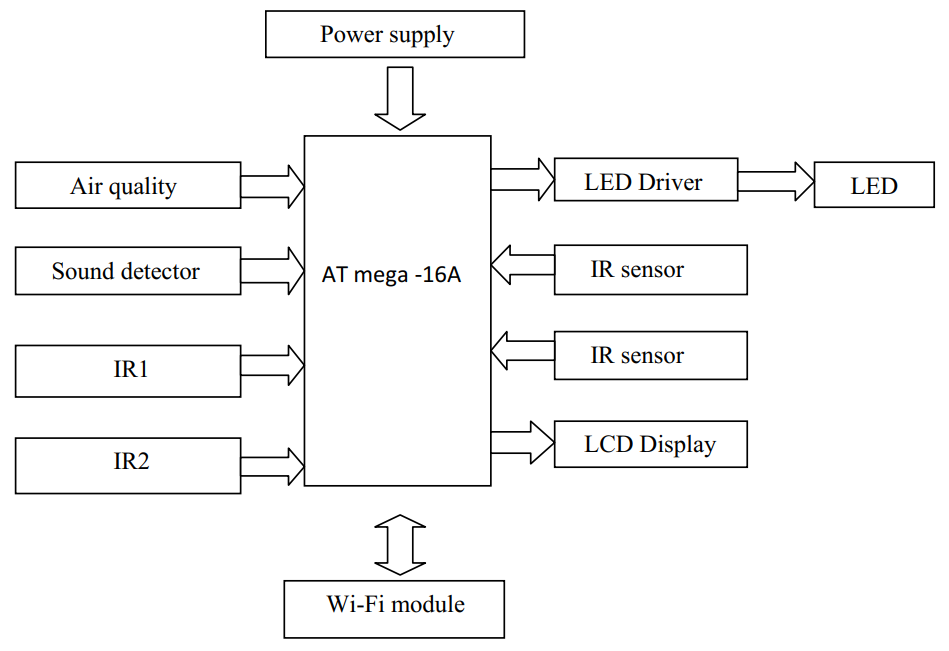
\includegraphics[scale=.5]{Capture.png}
	\end{center}
	
	
	
	\section*{6. Future Research Possibilities on Smart City:}
	We must be aware of the difference between immediate goals and long term viewpoints, when predicting the future work and expansion and application Smart City to build a Smart nation then we have to build smart cities to provide people a smart life. Thus the costing of building smart cities should reduce and the techniques and used devices should more efficient.
	
	\section*{7. Answering the Research Questions:}
	We conduct our survey with an aim to answer the three research questions described in section 2. In answer to the first research question we can say that we can describe the technique in subsections 5.1 to 5.5 mention these
	technique. Our discussions demonstrate the extent to which each of these categories has been explored. We have also tried to provide possible suggestions for further exploration.
	In answer to our second research question we can state that we have identified Zigbee as a solution and in section 5 in subsection 5.6 the features of zigbee has been described. Our study findings can be helpful for
	researchers aiming to explore the area of IoT based Smart City.
	
	
	\section*{8. Conclusion}
	The Smart city mission will drive economic growth and improve the quality of life of people and enable
	development of local areas. It will help connect technology which will lead to smart outcomes.
	In the Smart Energy Saver Street light is a cost effective, practical, eco-friendly and the safest way to save energy
	and this system the light status information can be accessed from anytime and anywhere. It clearly outfit the two
	problems that world is facing today, saving of energy and also management of incandescent lamps very
	efficiently.
	The Automatic Air and Sound management system is a step forward to provide a answer to the biggest threat. It
	supports the new technology and effectively supports the healthy life concept. This system has features for the
	common man to monitor the aggregate of pollution on their mobile phones using the application. Future investigations in this direction will add much value to smart city implementation.
	We also feel the necessity of future research towards ecofriendly, costfriendly and green smart city.
	
	\newpage
	
	\section{References}
	[1] L. Atzori, A. Iera, and G. Morabito, “The internet of things: A survey,”
	Comput. Netw., vol. 54, no. 15, pp. 2787–2805, 2010.
	\newline
	[2] P. Bellavista, G. Cardone, A. Corradi, and L. Foschini, “Convergence of
	MANET and WSN in IoT urban scenarios,” IEEE Sens. J., vol. 13, no. 10,
	pp. 3558–3567, Oct. 2013.
	\newline
	[3] A. Laya, V. I. Bratu, and J. Markendahl, “Who is investing in machine-tomachine communications?” in Proc. 24th Eur. Reg. ITS Conf., Florence,
	Italy, Oct. 2013, pp. 20–23.
	\newline
	[4] M. Dohler, I. Vilajosana, X. Vilajosana, and J. Llosa, “Smart Cities: An
	action plan,” in Proc. Barcelona Smart Cities Congress, Barcelona, Spain,
	Dec. 2011, pp. 1–6
	\newline
	[5]  I. Vilajosana, J. Llosa, B. Martinez, M. Domingo-Prieto, A. Angles, and
	X. Vilajosana, “Bootstrapping smart cities through a self-sustainable model
	based on big data flows,” IEEE Commun. Mag., vol. 51, no. 6, pp. 128–134,
	Jun. 2013
	\newline
	[6] T. Nuortio, J. Kytöjoki, H. Niska, and O. Bräysy, “Improved route planning
	and scheduling of waste collection and transport,” Expert Syst. Appl.,
	vol. 30, no. 2, pp. 223–232, Feb. 2006
	\newline
	[7] S. Lee, D. Yoon, and A. Ghosh, “Intelligent parking lot application using
	wireless sensor networks,” in Proc. Int. Symp. Collab. Technol. Syst.,
	Chicago, May 19–23, 2008, pp. 48–57
	\newline
	[8] N. Maisonneuve, M. Stevens, M. E. Niessen, P. Hanappe, and L. Steels,
	“Citizen noise pollution monitoring,” in Proc. 10th Annu. Int. Conf. Digital
	Gov. Res.: Soc. Netw.: Making Connec. Between Citizens, Data Gov., 2009,
	pp. 96–103.
	\newline
	[9]  J. P. Lynch and J. L. Kenneth, “A summary review of wireless sensors and
	sensor networks for structural health monitoring,” Shock and Vibration
	Digest, vol. 38, no. 2, pp. 91–130, 2006.
	\newline 
	[10] Pike research on Smart Cities [Online]. Available: http://www.pikeresearch.
	com/research/smart-cities
	
\end{document}
